%This work is licensed under the Creative Commons Attribution-NonCommercial-NoDerivs 3.0 United States License. To view a copy of this license, visit http://creativecommons.org/licenses/by-nc-nd/3.0/us/ or send a letter to Creative Commons, 444 Castro Street, Suite 900, Mountain View, California, 94041, USA.

To satisfy the first restriction, many of the common elements of an electron microscope column must be redesigned to accomodate the larger beam area.
I will then describe how we have addressed the necessity of the large-area source in building the prototype UEM system begin constructed at UIC.
In order to allow flexibility or to meet some technical challenges presented by the above considerations, much of the system is custom built.


\begin{figure}
  \centering
  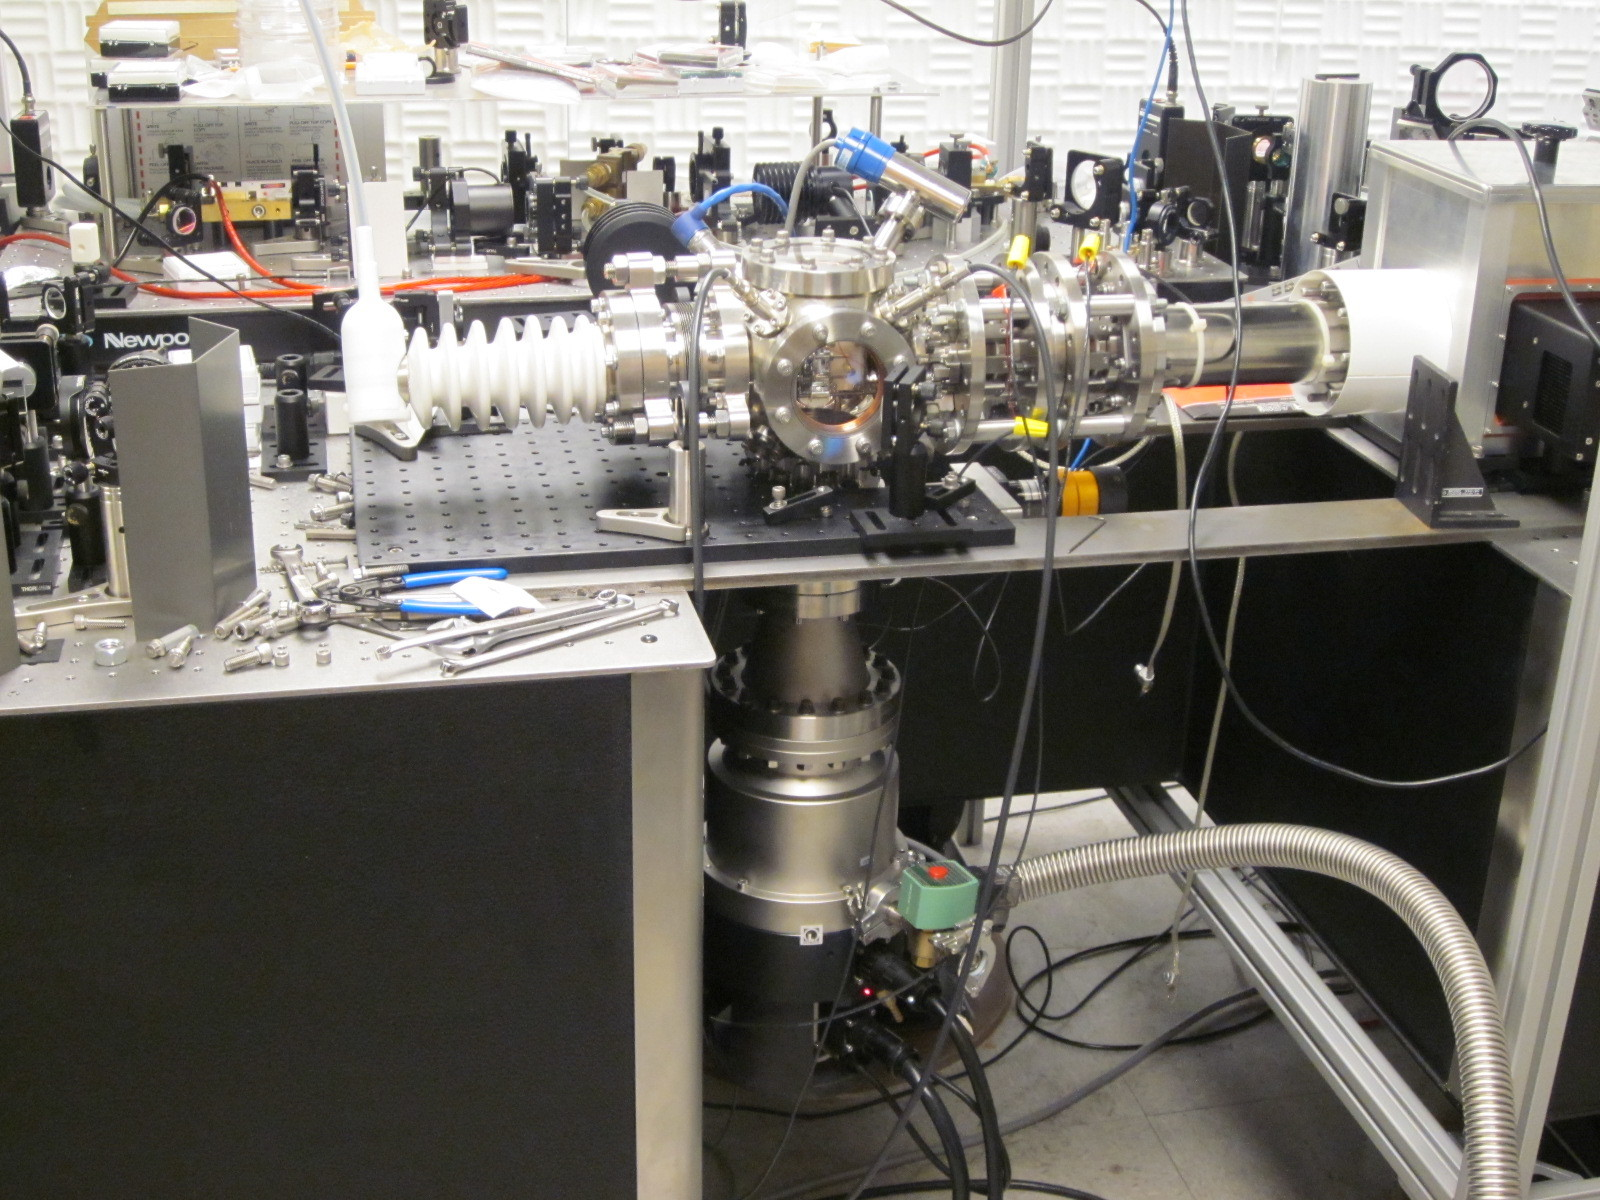
\includegraphics{inc/hardware/column.jpg}
  \caption[Picture of the prototype UEM column at UIC]{
    Picture of the majority of the prototype UEM column at UIC.
    The main vacuum chamber is laid sideways, with the high voltage (gun) at the left and the imaging system on the right.
    The magnetic levitated turbo pump hangs below the column, a scroll pump used for backing is not pictured.
    The laser system is in the background.
    All of the above is mounted on a custom shaped active vibration-canceling optical table.
    The electronic control systems are not pictured.
  }
  \label{fig:column-pic}
\end{figure}


